\appendix

\chapter{\textit{Source Code}}
	\textit{Source code} selengkapnya termasuk dengan \textit{data} 
	bisa dilihat di \url(https://github.com/EzraelVio/Fish-Viola-Jones) dibawah lisense 
	\textit{GNU General Public License v3.0.} \textit{Prototype System} Pendeteksi 
	Spesies Ikan Menggunakan \textit{Viola-Jones Featues Extraction} dan \textit{Boosting} 
	berbasis \textit{Decision Tree}.

\chapter{Tabel data \textit{training}}

\begin{longtable}{|c|c|c|c|c|}
    \hline
    \textbf{No.} & \textbf{Abudefduf} & \textbf{Amphiprion} & \textbf{Chaetodon} & \textbf{Negative} \\
    \hline
    \endfirsthead
    \multicolumn{5}{c}{{\tablename\ \thetable{} -- continued from previous page}} \\
    \hline
    \textbf{No.} & \textbf{Abudefduf} & \textbf{Amphiprion} & \textbf{Chaetodon} & \textbf{Negative} \\
    \hline
    \endhead
    \hline \multicolumn{5}{|r|}{{Continued on next page}} \\ \hline
    \endfoot
    \hline
    \endlastfoot

    1 & 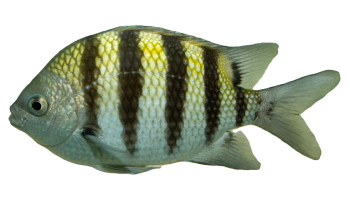
\includegraphics[width=3cm]{gambar/abudefduf/A1} & 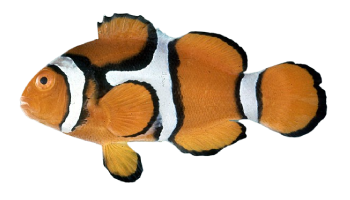
\includegraphics[width=3cm]{gambar/amphiprion/A1} & 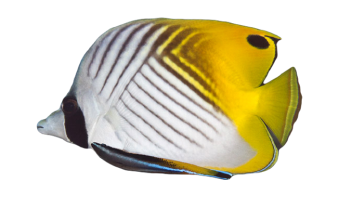
\includegraphics[width=3cm]{gambar/chaetodon/C1} & 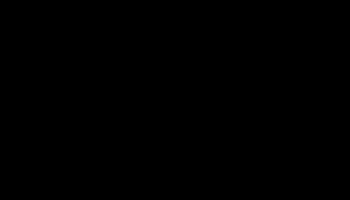
\includegraphics[width=3cm]{gambar/negative_examples/N1} \\
    \hline
    2 & 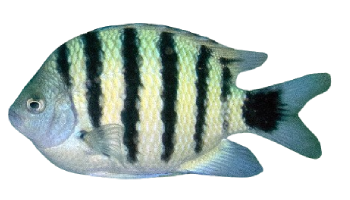
\includegraphics[width=3cm]{gambar/abudefduf/A2} & 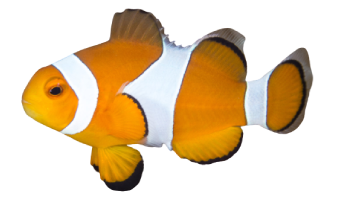
\includegraphics[width=3cm]{gambar/amphiprion/A2} & 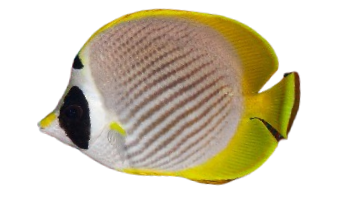
\includegraphics[width=3cm]{gambar/chaetodon/C2} & 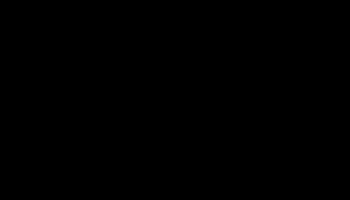
\includegraphics[width=3cm]{gambar/negative_examples/N2} \\
    \hline
    3 & 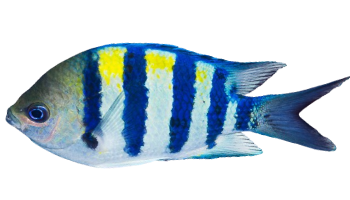
\includegraphics[width=3cm]{gambar/abudefduf/A3} & 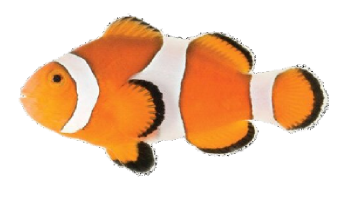
\includegraphics[width=3cm]{gambar/amphiprion/A3} & 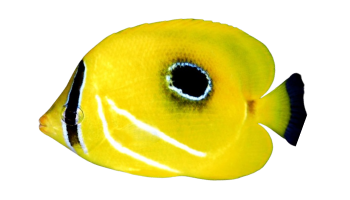
\includegraphics[width=3cm]{gambar/chaetodon/C3} & 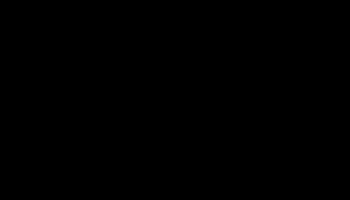
\includegraphics[width=3cm]{gambar/negative_examples/N3} \\
    \hline
    4 & 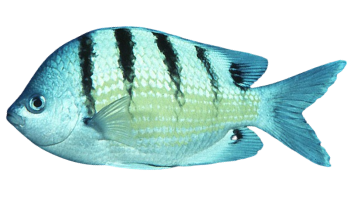
\includegraphics[width=3cm]{gambar/abudefduf/A4} & 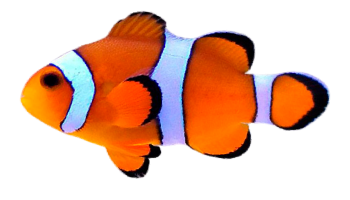
\includegraphics[width=3cm]{gambar/amphiprion/A4} & 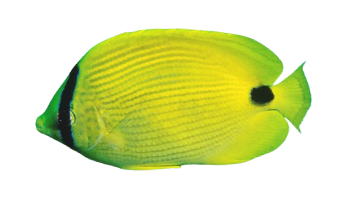
\includegraphics[width=3cm]{gambar/chaetodon/C4} & 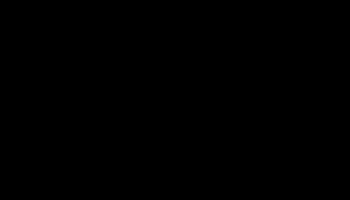
\includegraphics[width=3cm]{gambar/negative_examples/N4} \\
    \hline
    5 & 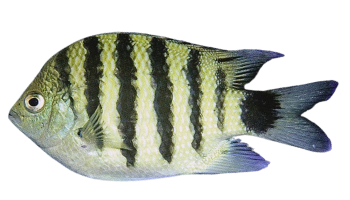
\includegraphics[width=3cm]{gambar/abudefduf/A5} & 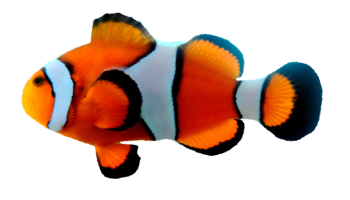
\includegraphics[width=3cm]{gambar/amphiprion/A5} & 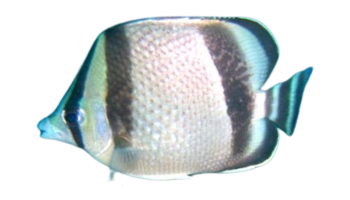
\includegraphics[width=3cm]{gambar/chaetodon/C5} & 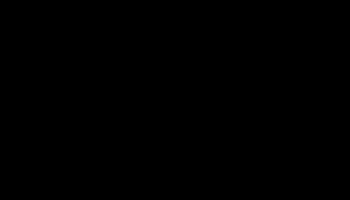
\includegraphics[width=3cm]{gambar/negative_examples/N5} \\
    \hline
    6 & 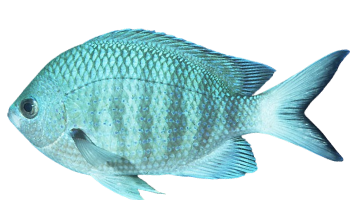
\includegraphics[width=3cm]{gambar/abudefduf/A6} & 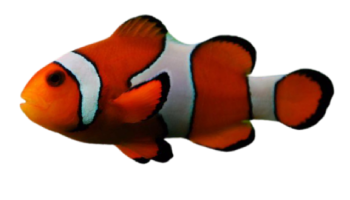
\includegraphics[width=3cm]{gambar/amphiprion/A6} & 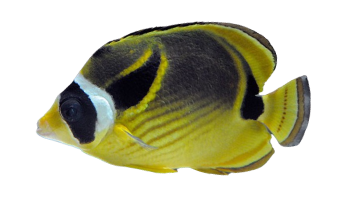
\includegraphics[width=3cm]{gambar/chaetodon/C6} & 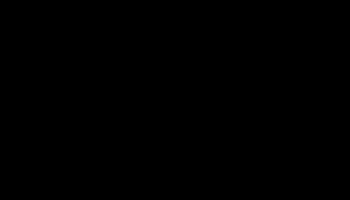
\includegraphics[width=3cm]{gambar/negative_examples/N6} \\
    \hline
    7 & 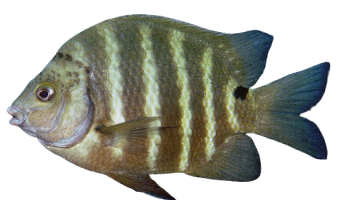
\includegraphics[width=3cm]{gambar/abudefduf/A7} & 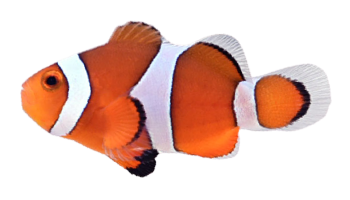
\includegraphics[width=3cm]{gambar/amphiprion/A7} & 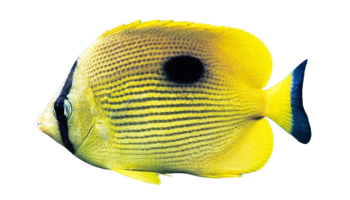
\includegraphics[width=3cm]{gambar/chaetodon/C7} & 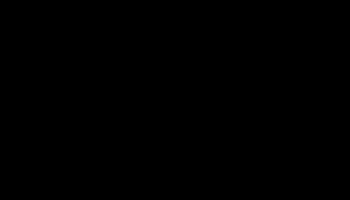
\includegraphics[width=3cm]{gambar/negative_examples/N7} \\
    \hline
    8 & 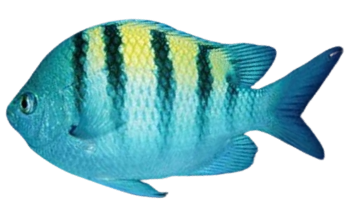
\includegraphics[width=3cm]{gambar/abudefduf/A8} & 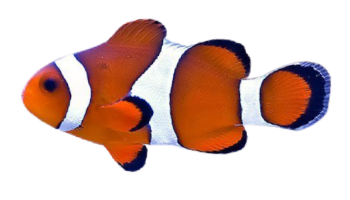
\includegraphics[width=3cm]{gambar/amphiprion/A8} & 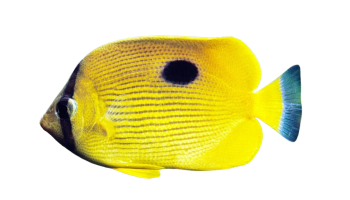
\includegraphics[width=3cm]{gambar/chaetodon/C8} & 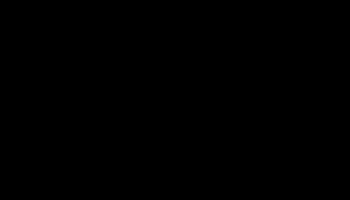
\includegraphics[width=3cm]{gambar/negative_examples/N8} \\
    \hline
    9 & 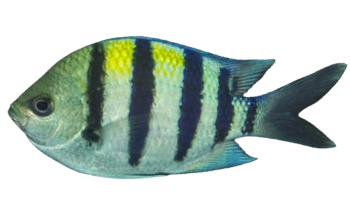
\includegraphics[width=3cm]{gambar/abudefduf/A9} & 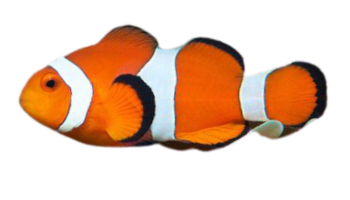
\includegraphics[width=3cm]{gambar/amphiprion/A9} & 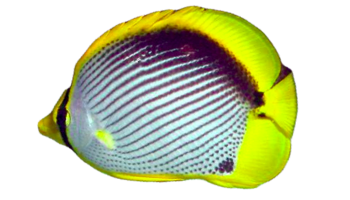
\includegraphics[width=3cm]{gambar/chaetodon/C9} & 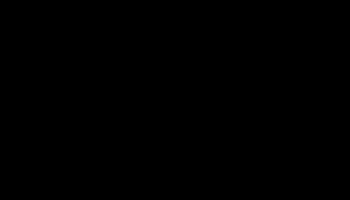
\includegraphics[width=3cm]{gambar/negative_examples/N9} \\
    \hline
    10 & 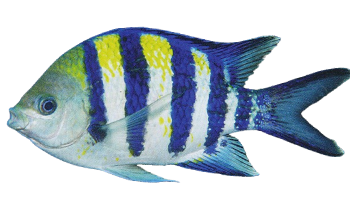
\includegraphics[width=3cm]{gambar/abudefduf/A10} & 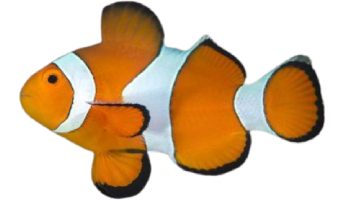
\includegraphics[width=3cm]{gambar/amphiprion/A10} & 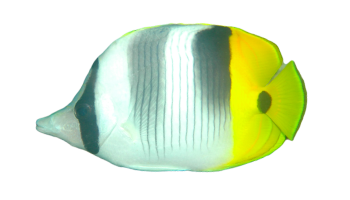
\includegraphics[width=3cm]{gambar/chaetodon/C10} & 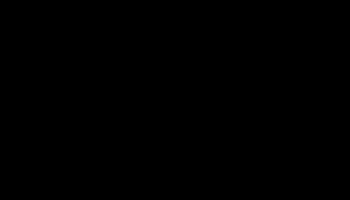
\includegraphics[width=3cm]{gambar/negative_examples/N10} \\
    \hline
    11 & 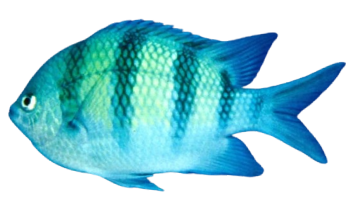
\includegraphics[width=3cm]{gambar/abudefduf/A11} & 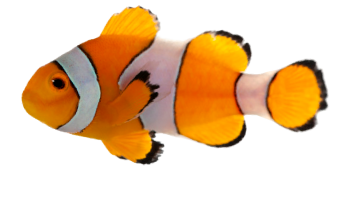
\includegraphics[width=3cm]{gambar/amphiprion/A11} & 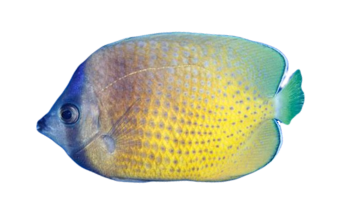
\includegraphics[width=3cm]{gambar/chaetodon/C11} & 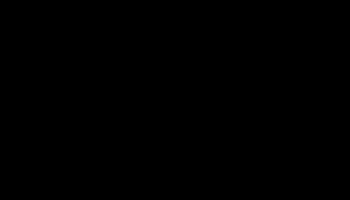
\includegraphics[width=3cm]{gambar/negative_examples/N11} \\
    \hline
    12 & 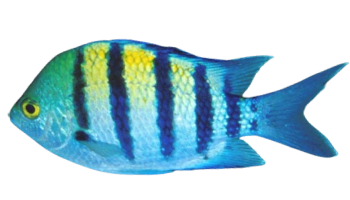
\includegraphics[width=3cm]{gambar/abudefduf/A12} & 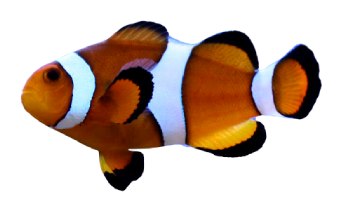
\includegraphics[width=3cm]{gambar/amphiprion/A12} & 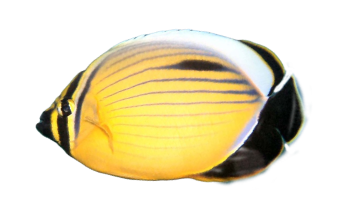
\includegraphics[width=3cm]{gambar/chaetodon/C12} & 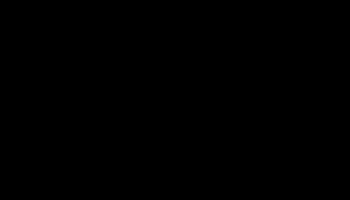
\includegraphics[width=3cm]{gambar/negative_examples/N12} \\
    \hline
    13 & 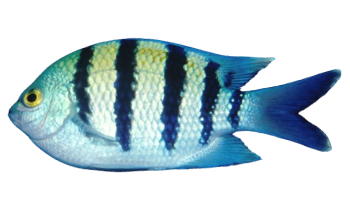
\includegraphics[width=3cm]{gambar/abudefduf/A13} & 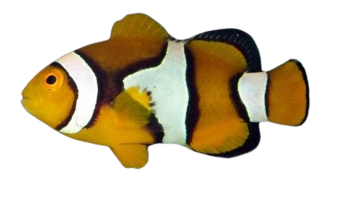
\includegraphics[width=3cm]{gambar/amphiprion/A13} & \includegraphics[width=3cm]{gambar/chaetodon/C13} & \includegraphics[width=3cm]{gambar/negative_examples/N13} \\
    \hline
    14 & \includegraphics[width=3cm]{gambar/abudefduf/A14} & \includegraphics[width=3cm]{gambar/amphiprion/A14} & \includegraphics[width=3cm]{gambar/chaetodon/C14} & \includegraphics[width=3cm]{gambar/negative_examples/N14} \\
    \hline
    15 & \includegraphics[width=3cm]{gambar/abudefduf/A15} & \includegraphics[width=3cm]{gambar/amphiprion/A15} & \includegraphics[width=3cm]{gambar/chaetodon/C15} & \includegraphics[width=3cm]{gambar/negative_examples/N15} \\
    \hline
    16 & \includegraphics[width=3cm]{gambar/abudefduf/A16} & \includegraphics[width=3cm]{gambar/amphiprion/A16} & \includegraphics[width=3cm]{gambar/chaetodon/C16} & \includegraphics[width=3cm]{gambar/negative_examples/N16} \\
    \hline
    17 & \includegraphics[width=3cm]{gambar/abudefduf/A17} & \includegraphics[width=3cm]{gambar/amphiprion/A17} & \includegraphics[width=3cm]{gambar/chaetodon/C17} & \includegraphics[width=3cm]{gambar/negative_examples/N17} \\
    \hline
    18 & \includegraphics[width=3cm]{gambar/abudefduf/A18} & \includegraphics[width=3cm]{gambar/amphiprion/A18} & \includegraphics[width=3cm]{gambar/chaetodon/C18} & \includegraphics[width=3cm]{gambar/negative_examples/N18} \\
    \hline
    19 & \includegraphics[width=3cm]{gambar/abudefduf/A19} & \includegraphics[width=3cm]{gambar/amphiprion/A19} & \includegraphics[width=3cm]{gambar/chaetodon/C19} & \includegraphics[width=3cm]{gambar/negative_examples/N19} \\
    \hline
    20 & \includegraphics[width=3cm]{gambar/abudefduf/A20} & \includegraphics[width=3cm]{gambar/amphiprion/A20} & \includegraphics[width=3cm]{gambar/chaetodon/C20} & \includegraphics[width=3cm]{gambar/negative_examples/N20} \\
    \hline
\end{longtable}

\chapter{Tabel pengolahan data gambar validasi}
Pada kolom \textit{Window} terdapat koordinat klasifikasi dan hasil klasifikasi. [6,110] class: 1 
berarti, 'dikasifikasikan di x = 6, y = 110 dengan hasil klasifikasi 1'.

\begin{longtable}{|c|c|c|c|c|}
	\hline
	\textbf{Image} & \textbf{Window 1} & \textbf{Window 2} & \textbf{Window 3} & \textbf{Final Result} \\
	\hline
	\endfirsthead
	\multicolumn{5}{c}{{\tablename\ \thetable{} -- continued from previous page}} \\
	\hline
	\textbf{Image} & \textbf{Window 1} & \textbf{Window 2} & \textbf{Window 3} & \textbf{Final Result} \\
	\hline
	\endhead
	\hline \multicolumn{5}{|r|}{{Continued on next page}} \\ \hline
	\endfoot
	\hline
	\endlastfoot
	\includegraphics[width=3cm]{gambar/dataset_validasi/Abudefduf01}
	& [6,110] class: 1 & [116,25] class: 1 & [233,41] class: 1 & Abudefduf \\
	\hline
	\includegraphics[width=3cm]{gambar/dataset_validasi/Abudefduf02}
	& [1,109] class: 3 & [116,30] class: 2 & [233,41] class: 1 & None \\
	\hline
	\includegraphics[width=3cm]{gambar/dataset_validasi/Abudefduf03}
	& [7,102] class: 3 & [116,33] class: 2 & [233,55] class: 2 & Abudefduf \\
	\hline
	\includegraphics[width=3cm]{gambar/dataset_validasi/Abudefduf04}
	& [5,105] class: 3 & [116,44] class: 3 & [233,55] class: 1 & Chaetodon \\
	\hline
	\includegraphics[width=3cm]{gambar/dataset_validasi/Abudefduf05}
	& [5,102] class: 2 & [116,39] class: 1 & [233,64] class: 2 & Amphiprion \\
	\hline
	\includegraphics[width=3cm]{gambar/dataset_validasi/Abudefduf06}
	& [8,107] class: 1 & [116,23] class: 1 & [233,40] class: 1 & Abudefduf \\
	\hline
	\includegraphics[width=3cm]{gambar/dataset_validasi/Abudefduf07}
	& [3,108] class: 1 & [116,36] class: 2 & [233,55] class: 1 & Chaetodon \\
	\hline
	\includegraphics[width=3cm]{gambar/dataset_validasi/Abudefduf08}
	& [23,110] class: 1 & [116,10] class: 2 & [233,35] class: 2 & Amphiprion \\
	\hline
	\includegraphics[width=3cm]{gambar/dataset_validasi/Abudefduf09}
	& [7,103] class: 2 & [116,22] class: 3 & [233,45] class: 1 & None \\
	\hline
	\includegraphics[width=3cm]{gambar/dataset_validasi/Abudefduf10}
	& [24,111] class: 1 & [116,11] class: 1 & [233,22] class: 1 & Abudefduf \\
	\hline
	\includegraphics[width=3cm]{gambar/dataset_validasi/Abudefduf11}
	& [10,102] class: 2 & [116,17] class: 2 & [233,40] class: 3 & Abudefduf \\
	\hline
	\includegraphics[width=3cm]{gambar/dataset_validasi/Abudefduf12}
	& [3,108] class: 1 & [116,29] class: 2 & [233,40] class: 3 & None \\
	\hline
	\includegraphics[width=3cm]{gambar/dataset_validasi/Abudefduf13}
	& [6,108] class: 1 & [116,42] class: 1 & [233,54] class: 1 & Abudefduf \\
	\hline
	\includegraphics[width=3cm]{gambar/dataset_validasi/Abudefduf14}
	& [6,108] class: 1 & [116,42] class: 3 & [233,54] class: 3 & Chaetodon \\
	\hline
	\includegraphics[width=3cm]{gambar/dataset_validasi/Abudefduf15}
	& [3,103] class: 1 & [116,33] class: 3 & [233,51] class: 3 & Chaetodon \\
	\hline
	\includegraphics[width=3cm]{gambar/dataset_validasi/Abudefduf16}
	& [0,110] class: 1 & [116,26] class: 2 & [233,59] class: 3 & None \\
	\hline
	\includegraphics[width=3cm]{gambar/dataset_validasi/Abudefduf17}
	& [6,102] class: 1 & [116,32] class: 2 & [233,50] class: 1 & Abudefduf \\
	\hline
	\includegraphics[width=3cm]{gambar/dataset_validasi/Abudefduf18}
	& [5,109] class: 1 & [116,28] class: 1 & [233,44] class: 1 & Abudefduf \\
	\hline
	\includegraphics[width=3cm]{gambar/dataset_validasi/Abudefduf19}
	& [8,99] class: 1 & [116,30] class: 1 & [233,59] class: 1 & Abudefduf \\
	\hline
	\includegraphics[width=3cm]{gambar/dataset_validasi/Abudefduf20}
	& [5,106] class: 1 & [116,27] class: 2 & [233,35] class: 1 & Abudefduf \\
	\hline
	\includegraphics[width=3cm]{gambar/dataset_validasi/Abudefduf21}
	& [8,102] class: 3 & [117,69] class: 3 & [233,54] class: 1 & Chaetodon \\
	\hline
	\includegraphics[width=3cm]{gambar/dataset_validasi/Abudefduf22}
	& [16,106] class: 1 & [116,23] class: 1 & [233,28] class: 1 & Abudefduf \\
	\hline
	\includegraphics[width=3cm]{gambar/dataset_validasi/Abudefduf23}
	& [7,112] class: 1 & [116,33] class: 2 & [233,58] class: 3 & None \\
	\hline
	\includegraphics[width=3cm]{gambar/dataset_validasi/Abudefduf24}
	& [10,108] class: 1 & [116,31] class: 3 & [233,42] class: 1 & Abudefduf \\
	\hline
	\includegraphics[width=3cm]{gambar/dataset_validasi/Abudefduf25}
	& [3,106] class: 3 & [116,29] class: 1 & [233,47] class: 2 & None \\
	\hline
	\includegraphics[width=3cm]{gambar/dataset_validasi/Amphiprion01} & [13,89] class: 1 & [116,12] class: 2 & [233,30] class: 2 & Amphiprion \\ \hline
	\includegraphics[width=3cm]{gambar/dataset_validasi/Amphiprion02} & [18,98] class: 1 & [116,26] class: 2 & [233,35] class: 3 & None \\ \hline
	\includegraphics[width=3cm]{gambar/dataset_validasi/Amphiprion03} & [15,95] class: 1 & [116,13] class: 2 & [233,27] class: 3 & None \\ \hline
	\includegraphics[width=3cm]{gambar/dataset_validasi/Amphiprion04} & [16,91] class: 1 & [116,0] class: 1 & [233,71] class: 1 & Abudefduf \\ \hline
	\includegraphics[width=3cm]{gambar/dataset_validasi/Amphiprion05} & [16,95] class: 2 & [116,23] class: 2 & [233,43] class: 3 & Amphiprion \\ \hline
	\includegraphics[width=3cm]{gambar/dataset_validasi/Amphiprion06} & [10,87] class: 1 & [116,9] class: 1 & [233,41] class: 1 & Abudefduf \\ \hline
	\includegraphics[width=3cm]{gambar/dataset_validasi/Amphiprion07} & [19,94] class: 1 & [116,31] class: 1 & [233,43] class: 1 & Abudefduf \\ \hline
	\includegraphics[width=3cm]{gambar/dataset_validasi/Amphiprion08} & [17,91] class: 1 & [116,0] class: 1 & [233,73] class: 1 & Abudefduf \\ \hline
	\includegraphics[width=3cm]{gambar/dataset_validasi/Amphiprion09} & [21,86] class: 1 & [116,17] class: 2 & [233,35] class: 1 & Abudefduf \\ \hline
	\includegraphics[width=3cm]{gambar/dataset_validasi/Amphiprion10} & [20,89] class: 2 & [116,20] class: 2 & [233,34] class: 2 & Amphiprion \\ \hline
	\includegraphics[width=3cm]{gambar/dataset_validasi/Amphiprion11} & [15,91] class: 1 & [116,10] class: 1 & [233,34] class: 1 & Abudefduf \\ \hline
	\includegraphics[width=3cm]{gambar/dataset_validasi/Amphiprion12} & [10,55] class: 1 & [116,17] class: 2 & [233,39] class: 3 & None \\ \hline
	\includegraphics[width=3cm]{gambar/dataset_validasi/Amphiprion13} & [17,93] class: 2 & [116,25] class: 2 & [233,46] class: 1 & Amphiprion \\ \hline
	\includegraphics[width=3cm]{gambar/dataset_validasi/Amphiprion14} & [18,89] class: 1 & [116,10] class: 1 & [233,28] class: 1 & Abudefduf \\ \hline
	\includegraphics[width=3cm]{gambar/dataset_validasi/Amphiprion15} & [14,93] class: 1 & [116,25] class: 2 & [233,33] class: 1 & Abudefduf \\ \hline
	\includegraphics[width=3cm]{gambar/dataset_validasi/Amphiprion16} & [21,94] class: 2 & [116,9] class: 1 & [233,19] class: 1 & Abudefduf \\ \hline
	\includegraphics[width=3cm]{gambar/dataset_validasi/Amphiprion17} & [15,96] class: 2 & [116,22] class: 2 & [233,37] class: 3 & Amphiprion \\ \hline
	\includegraphics[width=3cm]{gambar/dataset_validasi/Amphiprion18} & [16,91] class: 1 & [116,25] class: 2 & [233,37] class: 3 & None \\ \hline
	\includegraphics[width=3cm]{gambar/dataset_validasi/Amphiprion19} & [21,98] class: 3 & [116,10] class: 1 & [233,36] class: 1 & Abudefduf \\ \hline
	\includegraphics[width=3cm]{gambar/dataset_validasi/Amphiprion20} & [18,92] class: 1 & [116,8] class: 1 & [233,60] class: 2 & Abudefduf \\ \hline
	\includegraphics[width=3cm]{gambar/dataset_validasi/Amphiprion21} & [19,95] class: 1 & [116,0] class: 1 & [233,11] class: 1 & Abudefduf \\ \hline
	\includegraphics[width=3cm]{gambar/dataset_validasi/Amphiprion22} & [14,97] class: 3 & [116,32] class: 2 & [233,33] class: 1 & None \\ \hline
	\includegraphics[width=3cm]{gambar/dataset_validasi/Amphiprion23} & [19,88] class: 2 & [116,15] class: 2 & [233,28] class: 1 & Amphiprion \\ \hline
	\includegraphics[width=3cm]{gambar/dataset_validasi/Amphiprion24} & [12,89] class: 3 & [116,23] class: 1 & [233,72] class: 1 & Abudefduf \\ \hline
	\includegraphics[width=3cm]{gambar/dataset_validasi/Amphiprion25} & [14,87] class: 2 & [116,12] class: 1 & [233,36] class: 1 & Abudefduf \\ \hline
	\includegraphics[width=3cm]{gambar/dataset_validasi/Chaetodon01} & [32,116] class: 2 & [116,19] class: 1 & [233,19] class: 1 & Abudefduf \\ \hline
	\includegraphics[width=3cm]{gambar/dataset_validasi/Chaetodon02} & [35,118] class: 2 & [116,29] class: 1 & [233,40] class: 3 & None \\ \hline
	\includegraphics[width=3cm]{gambar/dataset_validasi/Chaetodon03} & [32,115] class: 1 & [116,30] class: 1 & [233,40] class: 3 & Abudefduf \\ \hline
	\includegraphics[width=3cm]{gambar/dataset_validasi/Chaetodon04} & [66,150] class: 0 & [116,57] class: 1 & [233,28] class: 1 & Abudefduf \\ \hline
	\includegraphics[width=3cm]{gambar/dataset_validasi/Chaetodon05} & [37,115] class: 1 & [116,28] class: 2 & [233,31] class: 2 & Amphiprion \\ \hline
	\includegraphics[width=3cm]{gambar/dataset_validasi/Chaetodon06} & [32,119] class: 2 & [116,26] class: 2 & [233,32] class: 1 & Amphiprion \\ \hline
	\includegraphics[width=3cm]{gambar/dataset_validasi/Chaetodon07} & [30,117] class: 1 & [116,24] class: 2 & [233,31] class: 1 & Abudefduf \\ \hline
	\includegraphics[width=3cm]{gambar/dataset_validasi/Chaetodon08} & [36,116] class: 2 & [116,17] class: 2 & [233,21] class: 3 & Amphiprion \\ \hline
	\includegraphics[width=3cm]{gambar/dataset_validasi/Chaetodon09} & [31,119] class: 1 & [116,18] class: 1 & [233,14] class: 2 & Abudefduf \\ \hline
	\includegraphics[width=3cm]{gambar/dataset_validasi/Chaetodon10} & [32,115] class: 1 & [116,27] class: 2 & [233,30] class: 1 & Abudefduf \\ \hline
	\includegraphics[width=3cm]{gambar/dataset_validasi/Chaetodon11} & [32,119] class: 1 & [116,23] class: 1 & [233,15] class: 1 & Abudefduf \\ \hline
	\includegraphics[width=3cm]{gambar/dataset_validasi/Chaetodon12} & [34,113] class: 1 & [116,21] class: 1 & [233,40] class: 3 & Abudefduf \\ \hline
	\includegraphics[width=3cm]{gambar/dataset_validasi/Chaetodon13} & [20,110] class: 1 & [116,21] class: 1 & [233,20] class: 2 & Abudefduf \\ \hline
	\includegraphics[width=3cm]{gambar/dataset_validasi/Chaetodon14} & [33,115] class: 2 & [116,33] class: 2 & [233,30] class: 1 & Amphiprion \\ \hline
	\includegraphics[width=3cm]{gambar/dataset_validasi/Chaetodon15} & [35,117] class: 1 & [116,26] class: 2 & [233,31] class: 2 & Amphiprion \\ \hline
	\includegraphics[width=3cm]{gambar/dataset_validasi/Chaetodon16} & [34,114] class: 1 & [116,28] class: 1 & [233,38] class: 1 & Abudefduf \\ \hline
	\includegraphics[width=3cm]{gambar/dataset_validasi/Chaetodon17} & [43,115] class: 1 & [116,23] class: 1 & [233,41] class: 1 & Abudefduf \\ \hline
	\includegraphics[width=3cm]{gambar/dataset_validasi/Chaetodon18} & [36,117] class: 1 & [116,23] class: 1 & [233,42] class: 1 & Abudefduf \\ \hline
	\includegraphics[width=3cm]{gambar/dataset_validasi/Chaetodon19} & [34,116] class: 1 & [116,21] class: 1 & [233,18] class: 1 & Abudefduf \\ \hline
	\includegraphics[width=3cm]{gambar/dataset_validasi/Chaetodon20} & [32,117] class: 2 & [116,40] class: 2 & [233,28] class: 1 & Amphiprion \\ \hline
	\includegraphics[width=3cm]{gambar/dataset_validasi/Chaetodon21} & [29,115] class: 1 & [116,30] class: 1 & [233,22] class: 1 & Abudefduf \\ \hline
	\includegraphics[width=3cm]{gambar/dataset_validasi/Chaetodon22} & [35,117] class: 2 & [116,22] class: 1 & [233,41] class: 1 & Abudefduf \\ \hline
	\includegraphics[width=3cm]{gambar/dataset_validasi/Chaetodon23} & [34,116] class: 1 & [116,24] class: 2 & [233,20] class: 2 & Amphiprion \\ \hline
	\includegraphics[width=3cm]{gambar/dataset_validasi/Chaetodon24} & [40,118] class: 1 & [116,22] class: 1 & [233,34] class: 2 & Abudefduf \\ \hline
	\includegraphics[width=3cm]{gambar/dataset_validasi/Chaetodon25} & [40,118] class: 1 & [116,12] class: 1 & [233,67] class: 1 & Abudefduf \\ \hline

	
	% Add more rows as needed
	\caption{Hasil prediksi menggunakan \emph{cascade} dan \emph{sliding window}}
	\label{tab: Classification result}
  \end{longtable}